 \documentclass[12pt,letterpaper]{article}

\usepackage{multicol}
\usepackage[x11names,table]{xcolor}
\usepackage{pstricks}
\usepackage{marginnote}
\usepackage[shortlabels]{enumitem}

\usepackage{parskip}
\usepackage{times}

%Configuracion del la hoja

\usepackage{geometry} %Paquete de margenes
\geometry{left=4cm, right=3cm, top=3cm, bottom=3cm}% Tamaño del área de escritura de la páginas
\usepackage{lscape}


%Paquetes para el entorno de escritura
\usepackage[spanish]{babel}
\usepackage[utf8]{inputenc} %Reconoce tildes y otros simbolos propios del español
\setlength\parindent{12pt}
\usepackage[breaklinks=true, hidelinks]{hyperref}


%Paquetes necesarios en el entorno cientifico
\usepackage{amsmath} %Paquete de smbología matemática de la American Mathematical Society.
\usepackage{amsfonts}%Paquete de smbología matemática de la American Mathematical Society.
\usepackage{amssymb}
\usepackage{latexsym}
\usepackage{graphicx} % Required for the inclusion of images
\usepackage{subfigure} % subfiguras
\usepackage{circuitikz} % Requerido para dibujar circuitos
\usepackage{tikz}
%\usepackage{siunitx} % Provides the \SI{}{} and \si{} command for typesetting SI units

%Paquetes para herramientas útiles en el desarrollo del texto
\usepackage{float}%Requerido para obligar a los elementos a colocarse donde uno quiera
\usepackage[final]{pdfpages} % util para agregar pdf al final del documento

%Paquetes para la bibliografia
\usepackage{natbib} % Requerido para cambiar bibliografia a formato APA
%\usepackage{cite}	
\usepackage{listings}


\renewcommand{\labelenumi}{\alph{enumi}.} % Make numbering in the enumerate environment by letter rather than number (e.g. section 6)


\usepackage{pgfgantt} %Cronograma de actividades

%----------------------------------------------------------------------------------------
%	PRESENTACION DEL DOCUMENTO
%----------------------------------------------------------------------------------------



\author{} % Author name

\date{31 de julio de 2019} % Date for the report

\begin{document}
	
	\renewcommand{\listfigurename}{Lista de Figuras}
	\renewcommand{\listtablename}{Lista de Tablas}
	\renewcommand{\contentsname}{Lista de Contenidos}
	\renewcommand{\figurename}{Figura}
	\renewcommand{\tablename}{Tabla}

	
 % Insert the title, author and date
\begin{center}

\vspace{3cm} ANTEPROYECTO \\

\vspace{8cm} DISEÑO DE UN SISTEMA DE ADQUISICIÓN Y TRANSMISIÓN DE DATOS ORIENTADO A MEDIDORES DE ENERGÍA ELÉCTRICA,UTILIZANDO UNA RED MALLADA WIFI CON MICROCONTROLADORES ESP32
\end{center}


\vspace{6cm}

\begin{flushleft}
	TUTOR ACADÉMICO: José Alonso. \\
	
\end{flushleft}

	
\begin{flushright}
	
	
		Presentado ante la ilustre\\
		Universidad Central de Venezuela\\
		por el BR. Marco Alejandro Rodríguez Ferrer \\
		para optar por el título de \\
		Ingeniero Electricista   \\
	


\end{flushright}


\vspace{2cm}
\thispagestyle{empty}
\newpage


\begin{center}
	\section*{ INTRODUCCIÓN}
\end{center}

Los primeros indicios del uso de la energía eléctrica sucedieron en el cuarto final del siglo XIX. La sustitución del gas y aceite por la electricidad además de ser un proceso técnico fue un verdadero cambio social que implicó modificaciones extraordinarias en la vida cotidiana de las personas, cambios que comenzaron por la sustitución del alumbrado público y posteriormente por varias clases de procesos industriales como motores, metalurgia, refrigeración y de último llegaron a las comunicaciones con la radio y la telefonía.\\

El siguiente cambio de paradigma en el que se vio involucrado la electricidad tuvo lugar a lo largo del siglo XX y surge desde la necesidad de facilitar las tareas realizadas a diario en casa. En ello los investigadores de la época vieron una solución adaptando equipos con energía eléctrica para su uso en el hogar. Las industrias replicaron el crecimiento tecnológico que tuvieron en sus productos, lo que trajo como consecuencia el desarrollo los electrodomésticos. La primera producción de aparatos en masa como refrigeradores, lavadoras, televisores y radios sucedieron en esta época y tuvieron una alta receptividad por parte de los compradores. La invención del transistor solo aceleró el reemplazo de aparatos dada su capacidad de minimizar los equipos.\\

La integración de la electrónica a la industria fomentó la creación de sistemas automatizados de adquisición de datos, supervisión y control también llamados sistemas \textit{SCADA} por sus siglas en inglés. Estos sistemas manejan áreas críticas de las industrias y son parte de los procesos fundamentales de muchas de ellas por lo que necesitan ser diseñados con robustez, fiabilidad y seguridad. La aparición del Internet y las comunicaciones modernas en estos sistemas permite a los usuarios, de manera inálambrica incluso, monitorear y actuar sobre el sistema a distancia, sin presencia física en la planta.\\

Además de poder monitorear y realizar acciones sobre los sistemas, los instrumentos de medida de última tecnología se fabrican de modo que puedan ser compatibles con medios de comunicación inalámbricas lo que posibilita la transmisión de datos adquiridos sin necesidad de cable a la central del sistema \textit{SCADA}. El presente trabajo de grado pretende realizar el diseño de un sistema de adquisición y transmisión de datos integrando microcontroladores ESP32 a medidores de energía eléctrica para formar una red mallada inalámbrica capaz de transmitir los datos recolectados a un punto central.

\newpage

		
\begin{center}
		\section*{ PLANTEAMIENTO DEL PROBLEMA}

\end{center}


\vspace{0.3cm}

La energía eléctrica es diferente de otras manifestaciones de la energía, debido a que no se puede almacenar por si sola como electricidad. Esto obliga a que la energía eléctrica consumida por un equipo u aparato tenga que generarse al momento en el cual se vaya a consumir. Los procesos para la generación de energía tienen costos altos de desarrollo e implementación a gran escala (países o estados) por lo que surtir de energía a las industrias y electrodomésticos tiene un costo que la empresa que genera la energía necesita recuperar. Como consecuencia se suele medir el consumo de cada uno de los usuarios por razones enteramente económicas.\\


En Venezuela se utiliza el mismo método de adquisición de datos desde que se instaló el sistema eléctrico. Este consiste en un operador que se acerca hasta el lugar donde se encuentra un medidor de energía y registra la lectura que marca el medidor, esto se hace de manera repetitiva para todos los sitios donde se quiera registrar el consumo. En ocasiones los medidores tienen una salida codificada donde comunica el valor del consumo por infrarrojo lo que permite al operador registrar el valor de ese consumo mediante un aparato compatible con este protocolo. Debido a esta problemática surge la necesidad de sustituir este sistema de adquisición de datos manual por uno que no requiera el traslado del operador hasta el sitio, que sea económico, confiable y eficiente.\\


Los principales equipos de medición de energía poseen en su diseño una salida por pulsos y soportan distintos protocolos de comunicación, lo que representa una ventaja al trabajar con microcontroladores, pues estos son adaptables a la mayoría de los protocolos mediante programación lo que facilita la adquisición de los datos a partir del medidor. Por otra parte trabajar con microcontroladores ofrece la posibilidad de realizar comunicaciones inalámbricas si se adapta un módulo WiFi como periférico. Interconectar estos módulos WiFi para formar una red mallada permitiría la transmisión de los datos captados a una mayor distancia que la lograda por un único módulo y permitiría su salida hacia alguna red externa deseada sin utilizar cables entre los medidores y la central de adquisición de datos, y sin intervención presencial del operador. Ilustradas las debilidades expuestas anteriormente y las ventajas que representaría un sistema de este tipo se evidencia la necesidad de realizar el diseño.\\



 \newpage


 \begin{center}
 	\section*{JUSTIFICACIÓN}
 \end{center}

\vspace{1cm}

Una red mallada WiFi utilizando microcontroladores permite adaptar a la red equipos que soportan distintos métodos de extracción de datos; otorga la posibilidad de interconectar dispositivos mediante comunicaciones inalámbricas, que no poseen dicha capacidad originalmente; además su desarrollo permitiría extender las variables a medir y los métodos de adquisición de datos del sistema; y por último, posee bajos costos de instalación al no requerir de cableado entre los elementos de la red. \\

Establecer la red mallada se requiere de nodos que posean la capacidad de enlazarse entre sí formando redes de comunicación, además los nodos deben ser capaces de enrutar los mensajes donde viaja la información. Para un sistema de adquisición de datos es ideal que cada nodo de la red este conformado por un microcontrolador con un módulo WiFi integrado, esto permitiría que cada uno de los nodos extrajera los datos según el método que se requiera en cada fuente de datos y al formar parte de la red mallada se facilitaría la adquisición de datos para un sistema central. El ESP32 es una opción viable para esta aplicación debido a su módulo WiFi integrado y las librerias desarrolladas en comunicación vía WiFi, utilizar dicha tarjeta representa una ventaja económica y reduce los tiempos de desarrollo respecto a otros microcontroladores.

 \newpage


 \begin{center}
 	\section*{ANTECEDENTES}
 \end{center}

\vspace{1cm}

El concepto de una red mallada no es algo nuevo, consiste en una serie de dispositivos conectados todos entre sí con la capacidad de comunicarse y enviar datos a un lugar de destino. Las soluciones ya existentes que se tomarán como referencia han logrado: utilizar redes malladas de sensores que permiten una recolección y trasmisión de datos fuera de la red. Ademas se ha logrado comunicar de manera inalámbrica a dispositivos que originalmente no poseen esa facultad, equipando estos aparatos con módulos WiFi y un microcontrolador para el manejo del envío y recepción. Los trabajos mencionados se presentan a continuación:\\


El trabajo de los ingenieros \cite{RUIZ-AYALA2018} en el artículo ”Monitoreo de variables meteorológicas a través de un sistema inalámbrico de adquisición de datos” publicado en la Revista de investigación, desarrollo e innovación de Colombia. En este artículo se presenta el desarrollo de un sistema de monitoreo inalámbrico de variables climáticas. El diseño se realizó a partir de microcontroladores de Microchip, los cuales realizan la adquisición, almacenamiento y transmisión de las señales digitales. Se utilizó cinco canales para conexión con sensores, una memoria micro SD para el almacenamiento y un módulo WiFi para la supervisión inalámbrica de las variables. La información fue almacenada en una página web donde es posible consultar los datos, además se diseñó una aplicación de Android para visualización desde dispositivos móviles. El rendimiento en comparación con una estación meteorológica comercial fue satisfactorio. Se concluye que los microcontroladores son dispositivos adecuados para implementar sistemas de adquisición de datos que al ser combinados con aplicativos desarrollados, brindan soluciones competitivas a un costo razonable.\\


En cuanto al desarrollo realizado por el ingeniero \cite{DA2006} ”Diseño y construcción de un prototipo para medición y transmisión inalámbrica del consumo de energía eléctrica de un sistema monofásico bifilar” se abordó el diseño y la construcción de un dispositivo medidor (esclavo) y un dispositivo maestro. El dispositivo esclavo almacena distintas variables además de pares de energía-tiempo ordenados para generar información sobre la demanda. El esclavo es capaz de establecer comunicación bidireccional y responder a comandos para extracción de datos o configuración de parte del maestro. En caso de falla del suministro, el valor contador de energía se guarda en una memoria no volátil para su posterior recuperación. El hardware de medición de energía utiliza un chip ADE7753 de Analog Devices, en la comunicación inalámbrica se utiliza una radio de 433 MHz ATR-XTR-903 de ABACOM. El procesamiento queda a cargo de un PIC16F877A. El dispositivo maestro conectado al puerto serial del PC permite configurar al esclavo, visualizar y almacenar los datos de manera remota mediante una aplicación en el computador. La circuitería es idéntica a la del esclavo. Las pruebas de comunicación fueron satisfactorias permitiendo confirmar el funcionamiento de todas las características, con la limitación de 1 a 65535 esclavos, además se reservaron espacios de la trama para futuras ampliaciones.\\



\cite{QCGJ2018} en su trabajo ”Sistema De Monitoreo de Variables Medioambientales Usando Una Red de Sensores Inalámbricos y Plataformas De Internet De Las Cosas” se pensó en un sistema para la recolección de datos meteorológicos usando una red de sensores inalámbricos (RSI), capaz de transmitir datos en tiempo real. El sistema logró automatizar procesos de obtención de datos de manera continua y a largo plazo, por medio de un módulo de abastecimiento de energía solar que permite autonomía para su funcionamiento. Se propuso la utilización de dos sistemas: DigiMesh y WiFi. El procesamiento se realizó en un Arduino Uno, para la comunicación se utilizó un XBee PRO 900HP (DigiMesh) y un moduló Electric Imp.01 (WiFi). Adicionalmente se evaluó la transmisión de los datos hacia plataformas de Internet de las cosas (IoT), en donde se gestionará y visualizará los datos obtenidos por los nodos. Este sistema fue pensado como alternativa de bajo costo para sistemas meteorológicos y está basado en componentes de hardware y software libre. Al realizarse la validación de los datos obtenidos mediante un análisis estadístico con los datos registrados por una estación meteorológica se obtuvo un error relativo promedio máximo de 4,93 \%.\\








 \newpage


 \begin{center}
 	\section*{OBJETIVOS}
 \end{center}

\vspace{1cm}

\subsection*{OBJETIVO GENERAL}

Diseñar un sistema de adquisición y transmisión de datos orientado a medidores de energía eléctrica, utilizando una red mallada WiFi con microcontroladores ESP32.

\subsection*{OBJETIVOS ESPECÍFICOS}


\begin{enumerate}[1.]
	
	
	 \item Documentar los principales métodos de extracción de datos soportados por un medidor de energía, en particular, el protocolo Modbus por RS485 y la salida por pulsos.
	
	 \item Diseñar el módulo de programa para los nodos que componen la red mallada, conformados por microcontroladores ESP32
	
	 \item Adaptar un nodo para ser compatible con la salida por pulsos de un medidor de energía y almacenar el valor de la medida para su adquisición mediante la red.
	
	 \item Adaptar un nodo para adquirir datos desde un medidor de energía que soporte protocolo Modbus RTU vía RS485.
	
	 \item Validar el funcionamiento del sistema.
 	
\end{enumerate}
\newpage



\begin{center}
	
	\section*{ MARCO METODOLÓGICO}
	
\end{center}

\vspace{1cm}

Con la finalidad de realizar efectivamente cada objetivo del proyecto, se llevarán las siguientes metodologías:
\bigskip

\begin{enumerate}[1.]
	
	
	
	\item Documentación de los principales métodos de extracción de datos soportados por un medidor de energía, enfocándose en el protocolo Modbus por RS485 y la salida por pulsos
	
		\begin{enumerate}
		
		\item Investigación documental acerca de los principales métodos de extracción soportados por medidores. 
		
		\item Comparación de los métodos para extracción de datos desde un medidor según las ventajas que ofrecen al ser realizado desde un microcontrolador
		
		\item Selección del método de extracción de datos a ser utilizado en el sistema.
		
		
	\end{enumerate}
	
	\item  Diseño del módulo del programa para los nodos que componen la red mallada, conformados por microcontroladores ESP32.
	
	
	\begin{enumerate}
		
		\item Programación de la conectividad entre los nodos de la red
		
		\item Programación del Envío y recepción de mensajes internos en la red.
		
		\item Programación de la transmisión de los datos hacia el exterior.
		
		
		
	\end{enumerate}
	
	
	\item Adaptación del nodo para su compatibilidad con la salida por pulsos de un medidor de energía y almacenar el valor de la medida para su adquisición mediante la red.
	
	
	\begin{enumerate}
		
		\item Extracción de datos mediante detección de pulsos y almacenamiento en memoria volátil
		
		\item Almacenamiento de los datos en la memoria no volátil en caso de fallos en la alimentación.
		
		\item Compatibilidad como nodo de la red, para transmitir los datos captados.
		
	\end{enumerate}
	
	
	\item Adaptación de un nodo para la adquisición de datos desde un medidor de energía que soporte protocolo Modbus RTU vía RS485. 

	
	\begin{enumerate}
				
		\item Programación para el manejo del hardware externo al ESP32, capaz de recibir y transmitir datos por el bus RS485.
		
		\item Compatibilidad como nodo de la red, para transmitir los datos captados.
		
	\end{enumerate}


	
	\item Realización de pruebas para comprobar el funcionamiento del sistema.
	
	
	\begin{enumerate}
		
		\item Pruebas para comprobar el funcionamiento de la red mallada, reorganización y enrutamiento de la red en caso de la pérdida de comunicación entre nodos.
		
		\item Pruebas para comprobar la comunicación hacia el interior y exterior de la red mallada, así como la transmisión de los datos extraídos.
		
	\end{enumerate}
	
	
	
	
	
\end{enumerate}
	
	
\newpage
	
	
		\begin{center}
		
		\section*{ ALCANCE Y LIMITACIONES}	
	\end{center}
	
	El sistema de adquisición y transmisión de datos implementado es solo un prototipo, en el que se tendrán las siguientes limitantes:
		
	\begin{itemize}
	
	\item La red se compondrá de al menos cinco nodos interconectados entre sí mediante el módulo WiFi propio del ESP32.
	
	\item Habrá al menos un medidor con extracción de datos por salida de pulsos con carga y conectado a los nodos
	
	\item Al menos un nodo de la red es capaz de conectarse al exterior y transmitir los datos. 
	
	\item Habrá al menos un medidor con extracción de datos por RS485 conectado a los nodos, este medidor puede no tener carga. 
	
	\item Se contará con al menos un nodo como repetidor en la red.
	
	\item Los datos transmitidos serán mostrados en un software o terminal de computadora.
	
		
	\end{itemize}

	\begin{figure}[H]
		\centering
		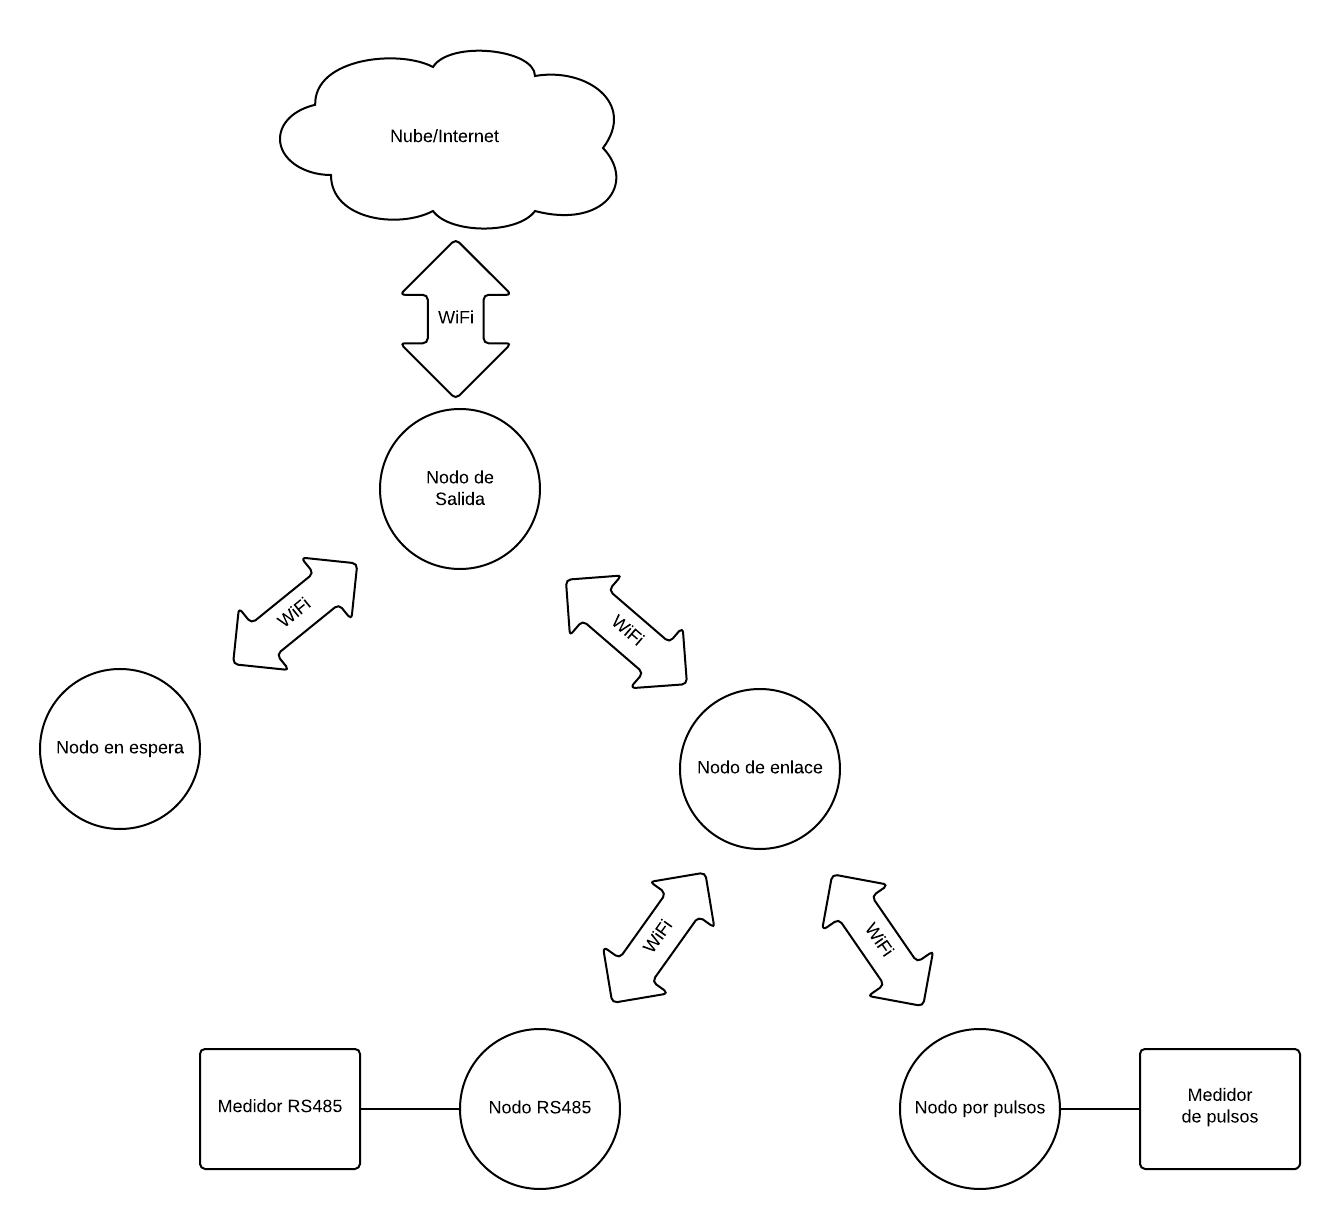
\includegraphics[width=0.7\linewidth]{EsquemaTEG}
		\caption{Representación gráfica de la red descrita en el alcance.}
		\label{fig:esquemateg}
	\end{figure}
	
	
	\newpage
	
	\begin{center}		
		\section*{ RECURSOS Y FACTIBILIDAD}	
	\end{center}

	Para el desarrollo e implementación del sistema se requiere de microcontroladores ESP32, medidores de consumo eléctrico y un computador para la instalación del IDE necesario para el desarrollo de aplicaciones en el microcontrolador.\\
	
	Tanto los microcontroladores ESP32 como los medidores de consumo de energía de tipo salida por pulsos o por RS485 serán suministrados por el tutor, ya se encuentran disponibles . El IDE (Interfaz de desarrollo) necesario para programar el ESP32 se encuentra en Github y tiene una documentación minuciosa escrita por los desarrolladores, además funciona en casi cualquier computador ya que no requiere de gran capacidad de cómputo.	\\
	
	
	
\newpage
	


	

	\begin{center}
		
		\section*{ CRONOGRAMA DE ACTIVIDADES}	



\vspace{0.5cm}
\resizebox{1.1\textwidth}{!}{
\begin{ganttchart}[
	canvas/.append style={fill=none, draw=black!5, line width=.75pt},
	hgrid style/.style={draw=black!5, line width=.75pt},
	vgrid={*1{draw=black!5, line width=.75pt}},
	today label font=\small\bfseries,
	title/.style={draw=none, fill=none},
	title label font=\bfseries\footnotesize,
	title label node/.append style={below=7pt},
	include title in canvas=false,
	bar label font=\mdseries\small\color{black!70},
	bar label node/.append style={left=.3cm},
	bar/.append style={draw=none, fill=black!63},
	bar incomplete/.append style={fill=blue},
	bar progress label font=\mdseries\footnotesize\color{black!70},
	group incomplete/.append style={fill=blue},
	group left shift=0,
	group right shift=0,
	group height=.5,
	group peaks tip position=0,
	group label node/.append style={left=.3cm},
	group progress label font=\bfseries\small,
	link/.style={-latex, line width=1.5pt, red},
	link label font=\scriptsize\bfseries,
	link label node/.append style={below left=-2pt and 0pt},
	]{1}{24}
	\gantttitle{Diseñar un sistema de adquisición y transmisión de datos orientado a medidores}{24} \\
	\gantttitle{de energía eléctrica utilizando una red mallada WiFi con microcontroladores ESP32.}{24} \\[grid]
	\gantttitle[
	title label node/.append style={below left=7pt and -3pt}
	]{Semana:\quad1}{1}
	\gantttitlelist{2,...,24}{1} \\
	\ganttgroup{Documentar métodos de extracción}{1}{3} \\
	\ganttbar{\textbf{Investigación Documental}}{1}{1} \\
	\ganttbar{\textbf{Comparación de métodos}}{2}{2} \\
	\ganttbar{\textbf{Selección de métodos}}{3}{3} \\
	\ganttgroup{Diseño del módulo para red mallada}{4}{10} \\
	\ganttbar{\textbf{Conectividad entre nodos}}{4}{6} \\
	\ganttbar{\textbf{Comunicación interna}}{7}{8} \\
	\ganttbar{\textbf{Comunicación externa}}{9}{10} \\
	\ganttgroup{Compatibilidad con salida por pulsos}{11}{15} \\	
	\ganttbar{\textbf{Extracción de datos}}{11}{12} \\
	\ganttbar{\textbf{Almacenamiento en memoria no volátil}}{13}{14} \\
	\ganttbar{\textbf{Comunicación interna con la red}}{15}{15} \\
	\ganttgroup{Compatibilidad con Modbus RTU RS485}{16}{20} \\
	\ganttbar{\textbf{Manejo de bus RS485}}{16}{18} \\
	\ganttbar{\textbf{Comunicación interna con la red}}{19}{20} \\
	\ganttgroup{Pruebas de funcionamiento}{21}{24} \\	
	\ganttbar{\textbf{Pruebas de reorganización y enrutamiento}}{21}{22} \\
	\ganttbar{\textbf{Comunicación interna y externa de la red}}{23}{24} \\
\end{ganttchart}
}

	\end{center}

\newpage

\bibliographystyle{apalike}
\bibliography{Marco_Rodriguez_Anteproyecto}

\end{document}

